% --- PREÂMBULO E PACOTES ---
\documentclass[12pt, a4paper]{article}
\usepackage[utf8]{inputenc}
\usepackage[T1]{fontenc}
\usepackage[brazil]{babel}
\usepackage{geometry}
\usepackage{indentfirst}
\usepackage{setspace}
\usepackage{titlesec}
\usepackage{graphicx}
\usepackage{amsmath}
\usepackage{hyperref}
\usepackage[alf,abnt-numeric-brackets]{abntex2cite}
\usepackage{booktabs}
\usepackage{float}
\usepackage{footnote}
\usepackage{array}
\usepackage{tabularx}
\usepackage{ragged2e}
\usepackage{fancyhdr}
\usepackage{longtable}
\usepackage{tabularx}

% Configurações de formatação 
\onehalfspacing
\setlength{\parindent}{1cm}
\titleformat{\section}{\normalfont\bfseries}{\thesection}{1em}{}

% Margens 
\geometry{
    a4paper,
    left=3.5cm,
    right=3.5cm,
    top=2.5cm,
    bottom=2.5cm,
    headheight=1cm,
    footskip=0cm
}

% --- CONFIGURAÇÕES PARA NUMERAÇÃO DE PÁGINA ---
\pagestyle{empty}
\fancyhf{}
\fancyhead[R]{\thepage}
\renewcommand{\headrulewidth}{0pt}

\begin{document}

% --- CAPA ---
\begin{titlepage}
    \centering
    \vspace*{2cm}
    {\large PONTIFÍCIA UNIVERSIDADE CATÓLICA DO RIO DE JANEIRO\par}
    \vspace{2cm}
    {\LARGE \textbf{Identificação de datasets relacionados, em contexto com}\par} 
    {\LARGE \textbf{metadados ausentes ou parciais}\par} 
    \vspace{3cm}
    {\large \textbf{Sérgio Bernardelli Netto}\par} 
    \vfill
    {\large PROJETO FINAL DE GRADUAÇÃO\par} 
    \vspace{1cm}
    {\large CENTRO TÉCNICO CIENTÍFICO - CTC\par} 
    {\large DEPARTAMENTO DE INFORMÁTICA\par} 
    {\large Curso de Graduação em Ciência da Computação\par}
    \vspace{2cm}
    {\large Rio de Janeiro, Outubro de 2025\par} 
\end{titlepage}

% --- FOLHA DE ROSTO ---
\newpage
\begin{flushright}
    \includegraphics[width=0.15\textwidth]{logo-pucRio.png}
\end{flushright}

\vspace*{3cm}
\begin{center}
    {\large \textbf{Sérgio Bernardelli Netto}\par} 
    \vspace{2cm}
    {\LARGE \textbf{Identificação de datasets relacionados, em contexto com}\par} 
    {\LARGE \textbf{metadados ausentes ou parciais}\par} 
    \vspace{3cm}
    \begin{minipage}{0.8\textwidth}
        \singlespacing
        \small
        \centering
        Relatório de Projeto Final, apresentado ao\\ 
        programa Ciência da Computação da PUC-Rio\\ 
        como requisito parcial para a obtenção do título de\\
        Bacharel em Ciência da Computação.
    \end{minipage}
    \vspace{2cm}
    
    {\large Orientador: Marcos Vianna Villas\par} 
    \vfill
    {\large Rio de Janeiro, Outubro de 2025\par} 
\end{center}
\vspace{0.5cm}

% --- RESUMO E ABSTRACT ---
\newpage
\section*{Resumo}
\begin{singlespace}
\textbf{Bernardelli Netto, Sérgio. 
Vianna Villas, Marcos.} 
Identificação de datasets relacionados, em contexto com metadados ausentes ou parciais. 
Rio de Janeiro, \the\year.
20 p. Relatório de Projeto Final II -- Departamento de Informática. 
Pontifícia Universidade Católica do Rio de Janeiro.

\vspace{0.3cm}
O projeto irá propor metodologias e ferramentas para a análise, identificação e determinação de possíveis combinações de datasets, seja pela identificação de chaves estrangeiras entre dois datasets, seja pela similaridade entre datasets. 
Serão utilizadas técnicas de mineração de dados e aprendizado de máquina, entre outras. 
Os resultados obtidos pelo projeto poderão viabilizar novas análises de dados com a utilização de datasets que anteriormente não se apresentavam como relacionados, em um determinado contexto.

\vspace{0.3cm}

\textbf{Palavras-chave:} 
Identificação de datasets, metadados ausentes, metadados parciais, mineração de dados, aprendizado de máquina, dependências funcionais relaxadas, data lakes e automação de ligações 
\end{singlespace}

\section*{Abstract}
\begin{singlespace}
\textbf{Bernardelli Netto, Sérgio. 
Vianna Villas, Marcos.} 
Identification of Related Datasets in the Context of Missing or Partial Metadata. 
Rio de Janeiro, \the\year.

20 p. Relatório Final de Projeto Final II -- Departamento de Informática.
Pontifícia Universidade Católica do Rio de Janeiro.
\vspace{0.3cm}
This project proposes methodologies for analyzing, identifying, and determining potential combinations of datasets, focusing on the discovery of foreign keys or similarities between datasets with missing or partial metadata. 
The approach leverages data mining and machine learning techniques to automate the correlation process between tables. 
By doing so, the project aims to enable new forms of data analysis that were previously unattainable due to the lack of explicit relationships between datasets. 
The results are expected to enhance data integration and uncover insights in contexts where datasets appeared unrelated. 
\vspace{0.3cm}

\textbf{Keywords:} 
dataset identification, missing metadata, partial metadata, data mining, machine learning, relaxed functional dependencies, data lakes, and correlation automation 
\end{singlespace}

% --- AGRADECIMENTOS ---
\newpage
\section*{Agradecimentos} 

Agradeço primeiramente ao meu orientador, Professor Marcos Vianna Villas, pela orientação indispensável, paciência e pelas discussões técnicas que guiaram este trabalho desde a sua concepção até o protótipo final. 

Aos especialistas da área de dados que participaram das entrevistas, cuja "visão de mercado" foi crucial para direcionar o foco do projeto da teoria para uma aplicação prática e relevante. 

Aos meus pais, Paulo Marcos Gotardelo Fraga Moreira e Silvia Carla Bernardelli Fraga Moreira, pelo suporte incondicional que me forneceram e a quem dedico todo meu esforço. 

Aos amigos que conheci ao longo da faculdade, especialmente Lucas Caputo Bello, Isabella Carmo e Paulo Vitor Libório, que de colegas se tornaram inspirações. % 

A minha namorada, Maria Beatriz de Oliveira Rabello, pelo amor, compaixão e cuidado durante esta etapa complexa e ocupada. 
“Ich liebe dich”, amor. 

Por fim, agradeço a banca de professores que pôde participar desse processo, pelo tempo dedicado à análise deste trabalho, e pelas valiosas contribuições que contribuirão para a pesquisa. 

% --- SUMÁRIO E LISTAS ---
\newpage
\begin{singlespace}
\tableofcontents
\end{singlespace}

\listoffigures
% \addcontentsline{toc}{section}{Lista de Figuras}


% --- CONTEÚDO DO TRABALHO (Início) ---
\newpage
\pagenumbering{arabic}
\setcounter{page}{4}
\pagestyle{fancy}

\section{Introdução} 
\label{sec:introducao}

Com o aumento significativo da quantidade de dados disponíveis em diversos setores, a gestão eficiente e a correta interpretação desses dados se tornaram desafios cruciais. 
Em muitos cenários, os dados estão distribuídos em diferentes conjuntos de datasets, sejam eles tabelas pertencentes a um esquema de banco de dados tradicional ou arquivos armazenados em data lakes1, sendo estes representações de uma abordagem alternativa aos armazéns de dados tradicionais, permitindo o armazenamento de dados em sua forma original e sem a necessidade de esquemas rígidos. 
No entanto, essa flexibilidade também traz desafios significativos, como a possibilidade de o repositório se tornar um data swamp, com dados de difícil organização e acesso sem metadados robustos. 
As tabelas de um esquema de banco de dados geralmente contam com chaves estrangeiras (FKs) previamente definidas, o que facilita a identificação da relação entre elas. 
No entanto, em ambientes de data lakes, onde os dados são frequentemente ingeridos sem metadados adequados, a situação é mais complexa. 
Quando esses data lakes carecem de organização e descrição de seus dados, transformam-se em verdadeiros data swamps, dificultando a identificação de ligações entre conjuntos de dados. 
Data lakes representam uma abordagem alternativa aos armazéns de dados tradicionais, permitindo o armazenamento de dados em sua forma original e sem a necessidade de esquemas rígidos. 
No entanto, essa flexibilidade também traz desafios significativos, como a possibilidade de o repositório se tornar um data swamp, com dados de difícil organização e acesso sem metadados robustos (Khine \& Wang, 2018). 
A falta de metadados estruturados, seja em tabelas de bancos de dados com FKs ou em data lakes, representa um obstáculo crítico para a identificação de ligações entre datasets. 
Sem esses metadados, relacionar as informações se torna uma tarefa manual e propensa a erros, especialmente quando se lida com grandes volumes de dados dispersos. 
Portanto, a falta de metadados é um problema real que impede o aproveitamento total das potencialidades dos dados, limitando a capacidade de realizar análises aprofundadas. 
A ausência de mecanismos automatizados para identificar possíveis combinações de datasets e chaves estrangeiras, assim como a similaridade entre datasets, afeta diretamente a qualidade das análises e a eficiência das operações de integração de dados. 

% --- SEÇÃO 2 ---
\newpage
\section{Situação Atual} 
\label{sec:situacao-atual}

A situação atual da automação da identificação de ligações entre bancos de dados envolve o uso de técnicas sofisticadas para otimizar a integração de dados, especialmente onde os metadados são limitados. 
Em sistemas legados, onde tabelas frequentemente não possuem chaves estrangeiras (FKs) definidas, ferramentas como o Metanome (Papenbrock et al., 2015) aplicam algoritmos avançados de perfilamento para detectar dependências complexas, como dependências de inclusão e funcionais. 
Nos data lakes, onde diversos datasets são colecionados sem uma descrição adequada, o problema se agrava. 
Para mitigar isso, o uso de dependências funcionais relaxadas (RFDs) estende as dependências clássicas para capturar ligações em dados não padronizados ou com inconsistências (Caruccio et al., 2016). 
No contexto de dados abertos, algoritmos de busca de similaridade, como o Locality Sensitive Hashing (LSH), oferecem soluções escaláveis para encontrar tabelas relacionáveis em bases amplas, como as governamentais (Bhardwaj et al., 2020). 
A literatura existente, embora robusta, frequentemente pressupõe um nível mínimo de metadados estruturais, como a presença de cabeçalhos (headers). 
Ferramentas como o Metanome, por exemplo, são altamente eficazes na descoberta de dependências, mas operam com maior eficácia quando o esquema dos dados, ou pelo menos os nomes dos atributos, são conhecidos. 
Este trabalho posiciona-se de forma complementar a essas soluções, focando em um nicho específico e desafiador: o data lake em seu estado mais bruto, onde até mesmo os cabeçalhos das colunas podem estar ausentes. 
A metodologia desenvolvida (detalhada na Seção 4), especialmente a partir do Protótipo 4, foi projetada para ser resiliente a essa degradação de metadados. 
Ao validar sistematicamente a capacidade do sistema de inferir relações em arquivos sem cabeçalho (usando dados sintéticos) e, posteriormente, generalizar essa lógica para dados reais e desconhecidos do gov.br (Protótipo 5), este projeto oferece uma contribuição prática.
A solução final atua como uma ferramenta de perfilagem e descoberta ágil na "primeira milha" da ingestão de dados, preparando o terreno para que ferramentas de análise mais profundas, como as citadas, possam ser aplicadas de forma eficaz em um momento posterior. 

% --- SEÇÃO 3 ---
\newpage
\section{Objetivos} 
\label{sec:objetivos}

O principal objetivo deste trabalho é propor metodologias e ferramentas que automatizem a análise, identificação e determinação de possíveis combinações entre diferentes datasets, mesmo em contextos onde os metadados estejam ausentes ou sejam parciais. 
Especificamente, o projeto visa desenvolver soluções que permitam a identificação de chaves estrangeiras entre dois ou mais datasets, bem como a detecção de similaridades que possam indicar possíveis ligações entre tabelas ou arquivos de dados. 
Espera-se que os resultados obtidos viabilizem novas formas de análise de dados, permitindo explorar ligações ocultas ou não evidentes entre datasets que, anteriormente, não se apresentavam como conectados, promovendo assim uma análise mais abrangente e integrada. 

% --- SEÇÃO 4 ---
\newpage
\section{Desenvolvimento de Protótipos} 
\label{sec:desenvolvimento-prototipos}

Para atender aos objetivos do projeto, optou-se por uma metodologia de desenvolvimento iterativa, estruturada em cinco protótipos. 
Esta abordagem foi escolhida para permitir a validação e o refinamento progressivo da complexidade algorítmica, com cada protótipo construindo sobre as lições aprendidas na iteração anterior. 

\subsection{Especificação}
\label{subsec:especificacao}

O escopo de cada protótipo foi definido de forma incremental: o Protótipo 1 (P1) visava validar a lógica de perfilamento de arquivo único. 
O Protótipo 2 (P2) tinha como escopo introduzir o "segundo algoritmo" de inferência relacional. 
O Protótipo 3 (P3) focou na "visão de mercado", implementando uma API para integração.
O Protótipo 4 (P4) foi desenhado para testar a robustez do "quarto algoritmo" contra dados degradados (ex: sem cabeçalho).
Por fim, o Protótipo 5 (P5) teve como escopo validar a generalização do sistema final em um domínio de dados real e desconhecido.
A solução foi especificada para ser desenvolvida integralmente na linguagem Python (versão 3.11), escolhida por sua robustez e pelo vasto ecossistema de bibliotecas para ciência de dados.
A arquitetura de software foi planejada para ser modular, com uma clara separação entre a lógica de orquestração (src/main.py), os componentes de análise (src/components/) e os módulos de utilidade (src/utils/).
Para a Ingestão de Dados, a especificação definiu o uso da biblioteca glob para a descoberta de arquivos de forma dinâmica e da biblioteca Pandas para a leitura de arquivos CSV (pandas.read\_csv), devido à sua eficiência e capacidade de lidar com diversos formatos e codificações.
Para o Perfilamento, foi especificado o uso de operações nativas da biblioteca Pandas para o cálculo de metadados estatísticos, como .dtype para tipos de dados, .nunique() para contagem de valores únicos, e .isnull().sum() para valores nulos.
Esta seria a base do componente DataProfiler.
Para o Matching de Atributos, a especificação previu o uso da biblioteca padrão difflib, especificamente a classe SequenceMatcher, para realizar a análise de similaridade textual entre nomes de colunas.
Esta abordagem foi escolhida por não requerer dependências externas e ser eficaz para a detecção de similaridade de strings.
Para a Inferência e Validação de Relações, o núcleo algorítmico do FKFinder, a especificação determinou o uso de estruturas de dados set (conjuntos) nativas do Python.
A verificação de inclusão de dados, a operação mais custosa do processo, seria implementada através do método issubset() (ou uma verificação percentual sobre ele), garantindo uma performance otimizada em comparação a iterações aninhadas.
Para a Integração de Sistema (escopo do P3), o micro-framework Flask foi especificado para a construção da API.
Sua leveza e facilidade em expor a lógica do sistema como endpoints HTTP que manipulam JSON foram os fatores decisivos.
Finalmente, para a Geração de Dados de Teste (escopo do P4), a especificação definiu a criação de um script (gerar\_dados\_artificiais.py) que utilizaria as bibliotecas Pandas e NumPy para criar datasets sintéticos com características controladas, permitindo testes de robustez em cenários de dados degradados.
A biblioteca logging padrão do Python foi definida como a ferramenta para registro de eventos e depuração em todas as fases.

% --- SEÇÃO 5 ---
\newpage
\section{Execução da Metodologia}
\label{sec:execucao-metodologia}

Esta seção detalha a execução da metodologia de desenvolvimento, documentando a especificação, construção, testes e ajustes de cada um dos cinco protótipos, conforme a "tabela" de avaliação sugerida.

\subsection{Protótipo 1: Prova de Conceito e Perfilamento de Arquivo Único} 
\label{subsec:prototipo1}

A Especificação do Protótipo 1 visava validar a lógica de perfilamento de arquivos isolados. 
O sistema foi projetado para ser executado como um script de linha de comando (python src/main.py). 
O fluxo de utilização era o seguinte: o usuário deveria popular o diretório /datasets/ com arquivos .csv. 
Ao ser executado, o script (prototipo 1/src/main.py) utilizaria o FileHandler para encontrar todos os arquivos, o DataLoader para carregá-los um a um, e o DataProfiler para analisá-los. 
O sistema então imprimiria no console os metadados estatísticos (tipo, nulos, únicos) de cada coluna e uma lista de Chaves Primárias (PKs) candidatas para cada arquivo. 
A saída era um relatório textual (results/attribute\_suggestions.txt). A especificação não incluía qualquer forma de análise relacional entre os arquivos. 
A Construção desta fase foi realizada em Python 3.11, com a biblioteca Pandas sendo a principal dependência para ingestão e análise, conforme a especificação tecnológica. 
O componente central foi o DataProfiler (src/components/data\_profiler.py), que continha a lógica de cálculo de métricas e a regra de negócio para identificar uma PK (baseada em limiares de unicidade e não nulidade).
Os módulos FileHandler (src/utils/file\_handler.py) e DataLoader (src/utils/data\_loader.py) foram criados para abstrair a descoberta e o carregamento de arquivos. 
Os Testes do P1 foram executados utilizando um conjunto de dados real da NBA, obtido da plataforma Kaggle (datasets/). 
Os arquivos principais utilizados foram o Advanced.csv, contendo 26.280 linhas de estatísticas avançadas por jogador e temporada, e o Player Play By Play.csv, com 61.168 linhas de dados biográficos e estatísticas por jogo. 
O teste consistiu em executar o main.py e validar o relatório de saída.
O sistema foi bem-sucedido em carregar ambos os arquivos e identificar corretamente as PKs candidatas (como seas\_id em Advanced.csv) em cada arquivo de forma isolada, cumprindo a especificação. 
Os Ajustes necessários identificados no P1 foram puramente funcionais e arquiteturais. A avaliação confirmou a principal limitação: a ausência de análise relacional.
O sistema era "míope", incapaz de comparar os perfis entre si. 
O ajuste proposto para o Protótipo 2 foi, portanto, a criação de um novo componente, o FKFinder, e a refatoração completa do main.py para um fluxo em duas fases (profiling global seguido de análise relacional). 

\subsection{Protótipo 2: Inferência Relacional Básica} 
\label{subsec:prototipo2}

A Especificação do Protótipo 2 foi expandir a lógica para incluir o "segundo algoritmo", focado na inferência de Chaves Estrangeiras (FKs). 
O fluxo de utilização foi mantido (execução via python src/main.py), mas o comportamento do sistema foi fundamentalmente alterado. 
A nova especificação determinava que o main.py (src/main.py) deveria primeiro executar o DataProfiler em todos os arquivos, armazenando seus perfis em memória para criar um catálogo global de PKs candidatas. 
Em seguida, um novo componente, o FKFinder, deveria ser invocado para comparar cada coluna de cada tabela com este catálogo global. 
A lógica de inferência foi especificada para validar dois níveis: similaridade de metadados (tipo e nome) e inclusão de dados (conteúdo).
A saída do sistema foi modificada para gerar um novo artefato, output/fk\_identification\_results.txt, listando as relações de FK inferidas. 
A Construção reutilizou a base de código do P1, com a principal adição do FKFinder (src/components/fk\_finder.py). 
Conforme a especificação tecnológica, este componente utilizou a biblioteca difflib.SequenceMatcher (abstraída no AttributeMatcher (src/components/attribute\_matcher.py)) para a comparação de nomes. 
Para a validação de inclusão de dados, foi implementada uma lógica de verificação percentual sobre os conjuntos (set) de valores únicos da FK e da PK, garantindo performance. 
O main.py foi reescrito para orquestrar esse novo fluxo de duas fases. 
Os Testes desta fase utilizaram os mesmos datasets da NBA, porém, devido ao custo computacional da nova lógica de inclusão, foram utilizadas versões encurtadas para agilizar os ciclos de depuração. 
Mais importante, foi introduzido um conjunto de dados acadêmico (datasets/dataset - Copia/) com três tabelas (datasets\_teste\_tabela\_academica.csv, ...\_federal.csv, ...\_principal.csv) para validar a lógica de inferência em um domínio diferente.
Os testes confirmaram que o FKFinder conseguia, com sucesso, identificar a relação entre Advanced.csv e Player Play By Play.csv usando o seas\_id, e também inferir as relações corretas no conjunto acadêmico.
Os Ajustes identificados no P2 foram de duas naturezas. Primeiro, o desempenho da análise de inclusão, mesmo com sets, foi confirmado como um gargalo significativo em datasets maiores. 
Segundo, e mais importante, o sistema como um script local foi considerado de baixa usabilidade para um analista de dados.
O ajuste proposto para o Protótipo 3 foi focar na "visão de mercado", refatorando o sistema como um serviço de API para melhor integração e flexibilidade.

\subsection{Protótipo 3: Integração via API e Visão de Mercado} 
\label{subsec:prototipo3}

A Especificação do Protótipo 3 foi motivada pela "visão de mercado", identificada através de entrevistas com especialistas da área. 
O requisito era transformar a ferramenta de um script local em um serviço consumível. 
O sistema foi re-especificado para operar como uma API. O novo fluxo de utilização seria: o usuário iniciaria um servidor web (executando python api.py). 
Em seguida, utilizando qualquer cliente HTTP (como curl, Postman, ou um script), o usuário faria uma requisição POST para o endpoint /analyze. 
O corpo da requisição poderia conter parâmetros de configuração, como os limiares de validação. %
O sistema, então, executaria o pipeline completo (Profiling e FKFinder) e retornaria as relações encontradas em formato JSON. 
O fluxograma apresentado na Figura~\ref{fig:arquitetura_p3} ilustra esta arquitetura de sistema, que se tornou a base para as iterações subsequentes. 

\begin{figure}[H]
    \centering
    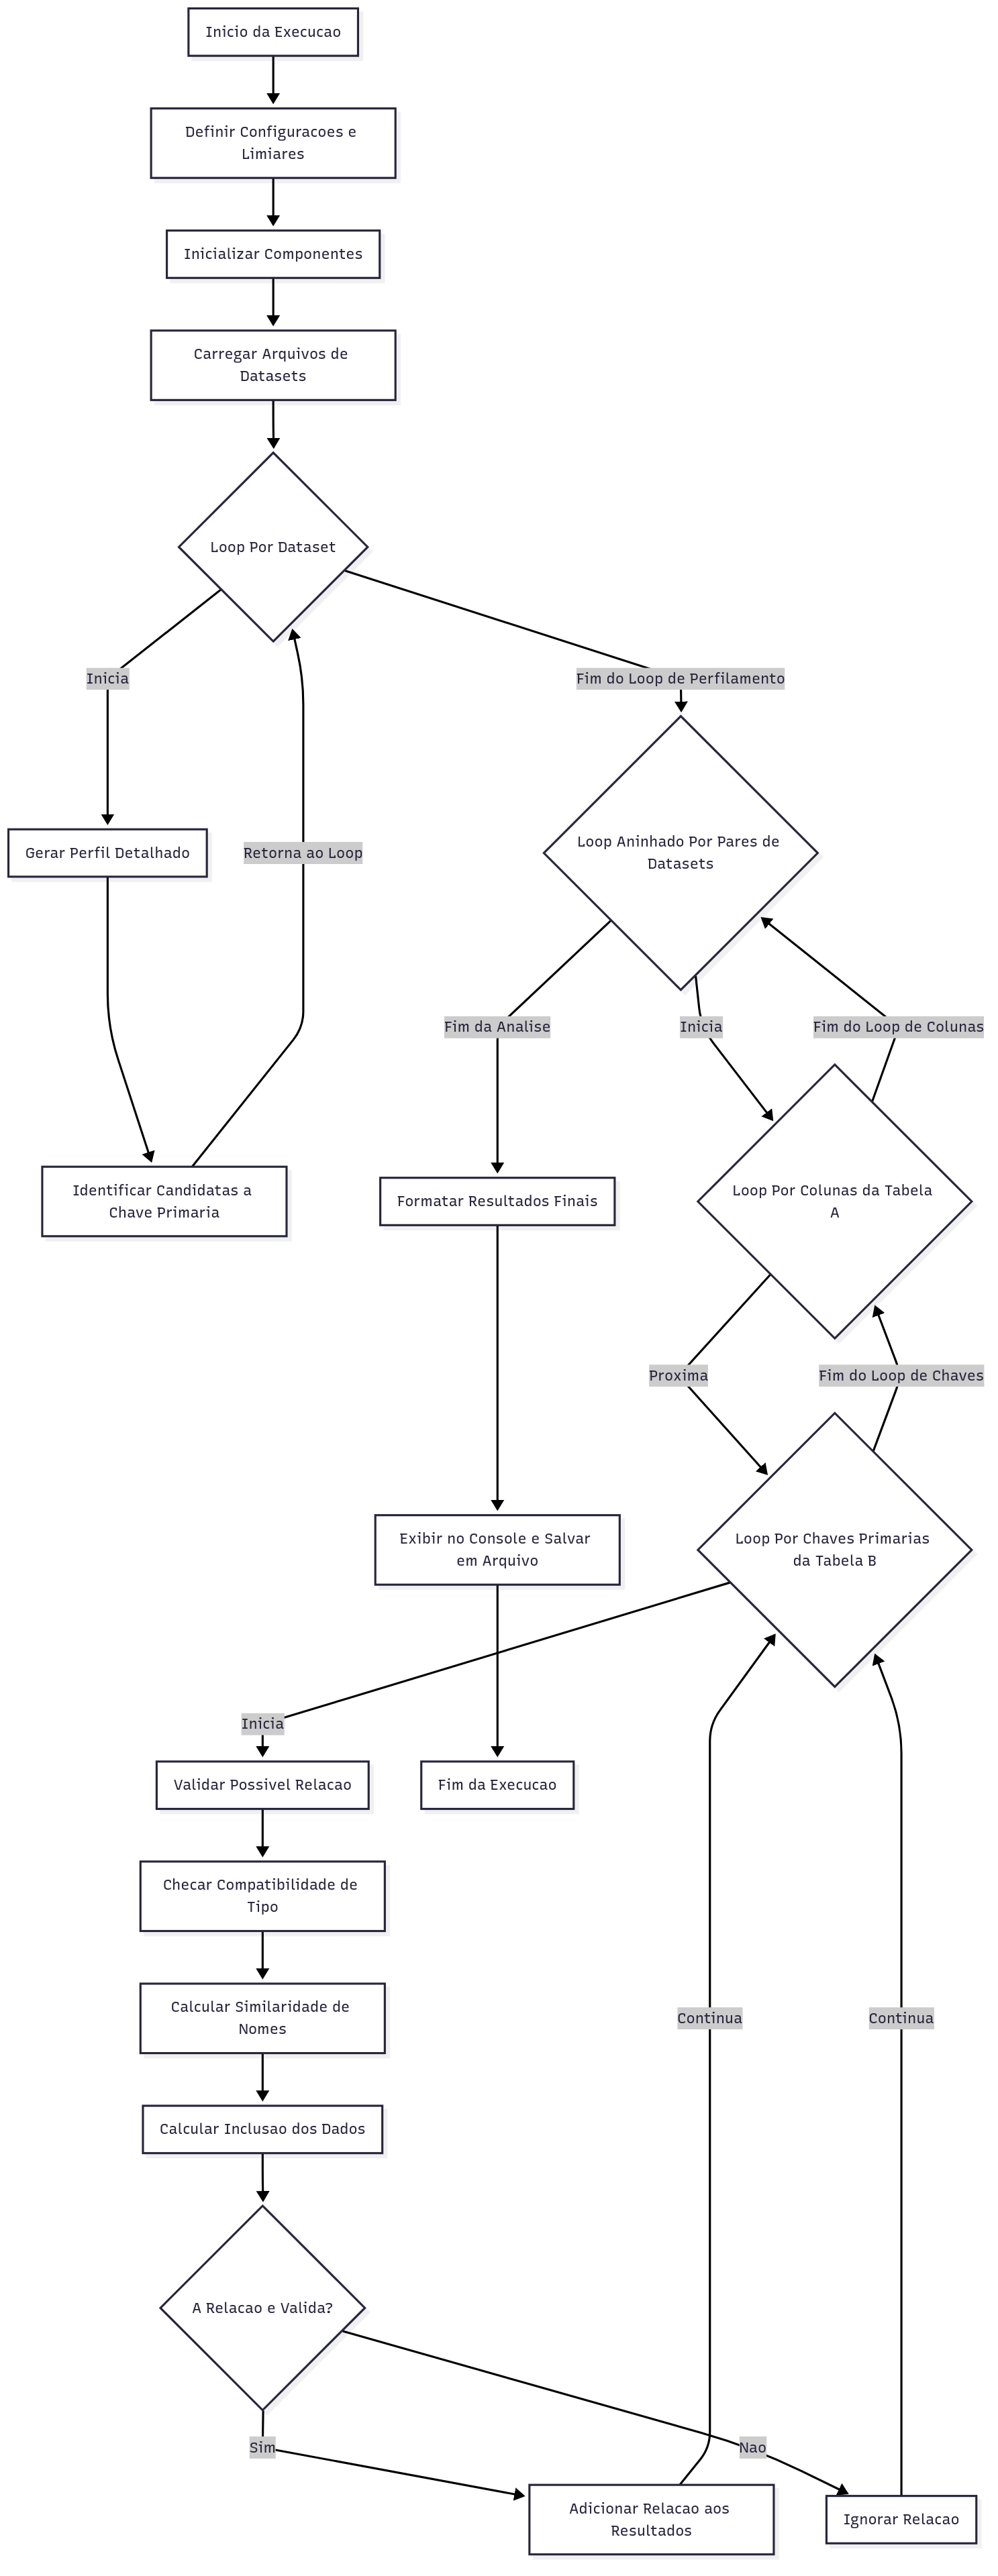
\includegraphics[width=0.65\textwidth]{Fluxograma tcc.png} 
    \caption{Arquitetura da API do Protótipo 3. (Documento de minha autoria.)}
    \label{fig:arquitetura_p3}
\end{figure}

A Construção do P3 introduziu a biblioteca Flask, conforme a especificação tecnológica. 
O novo arquivo api.py importou a lógica principal do main.py (que foi levemente refatorado para ser uma função analyze() reutilizável) e a "envolveu" em um endpoint de API. 
A biblioteca padrão logging foi configurada para fornecer feedback no console do servidor. 
O "terceiro algoritmo" foi um refinamento do FKFinder, expondo os limiares de validação (ex: inclusão, unicidade) como parâmetros na chamada da API, em vez de constantes no código, aumentando a flexibilidade do sistema. 
Os Testes desta fase foram primariamente qualitativos, baseados nas entrevistas com dois especialistas em análise de dados. 
O feedback validou que a abordagem de API era crucial para a adoção da ferramenta em ambientes corporativos. 
Testes de funcionalidade da API também foram realizados: o servidor Flask foi iniciado e requisições POST foram enviadas para o endpoint /analyze para validar que os parâmetros de entrada (limiares) eram processados corretamente e que a resposta JSON era formatada como esperado. 
Os Ajustes propostos após o P3 foram focados em robustez. As entrevistas e testes confirmaram que o sistema funcionava, mas os especialistas levantaram a preocupação sobre dados "sujos", muito comuns em data lakes. 
O sistema, em sua versão P3, ainda dependia de metadados de alta qualidade, como a presença de cabeçalhos (headers) para o AttributeMatcher funcionar. 
O ajuste necessário para o Protótipo 4 foi blindar o sistema contra cenários de degradação de metadados. 

\subsection{Protótipo 4: Robustez e Tratamento de Dados Degradados} 
\label{subsec:prototipo4}

A Especificação do Protótipo 4 foi unicamente de robustez. O objetivo era implementar o "quarto algoritmo", projetado para operar em cenários onde os metadados são parciais ou inexistentes. 
A especificação do DataLoader foi alterada para aceitar um parâmetro (via API) indicando a ausência de cabeçalho (header=None). 
A especificação do FKFinder foi alterada para não depender mais da similaridade de nomes como um filtro obrigatório; 
ele deveria ser capaz de inferir relações com base puramente no conteúdo (inclusão de dados). 
O fluxo de utilização para o usuário final (via API) permaneceu o mesmo do P3, mas com a adição de novos parâmetros na requisição JSON, como \{"header": false\}.
A Construção não envolveu novas bibliotecas. As modificações foram puramente lógicas no src/. 
O utils/data\_loader.py foi atualizado para interpretar o novo parâmetro da API e passá-lo para a função pandas.read\_csv (ex: pd.read\_csv(..., header=None)). 
A mudança mais importante foi no components/fk\_finder.py: a lógica foi alterada para que, caso a similaridade de nome (calculada pelo AttributeMatcher) fosse baixa ou nula, o algoritmo não descartasse a relação, mas sim prosseguisse para a validação de conteúdo (análise de inclusão), que passou a ser o critério decisivo. 
O script gerar\_dados\_artificiais.py (gerar\_dados\_artificiais.py) foi construído usando Pandas e NumPy para criar os datasets de teste sintéticos. 
Os Testes foram a parte crucial desta fase, utilizando os três conjuntos de testes sintéticos (datasets\_teste...). 
O primeiro, datasets\_teste1\_normais (ex: ALUNO.csv, MATRICULA.csv), validou o "caminho feliz" (dados limpos com cabeçalhos). 
O segundo, datasets\_teste2\_genericos (ex: ALUNO.csv, MATRICULA.csv com colunas col1, col2, etc.), forçou o FKFinder a ignorar o AttributeMatcher e funcionar apenas com a lógica de inclusão de conteúdo, o que foi um sucesso. 
O terceiro, datasets\_teste3\_sem\_cabecalho, testou o DataLoader e a capacidade do sistema de operar por índices de coluna, o que também foi validado. 
Os Ajustes identificados foram mínimos. Os testes sintéticos provaram que o "quarto algoritmo" era robusto em cenários controlados. 
A limitação final, no entanto, era que esta robustez ainda não havia sido testada em um ambiente real, complexo e desconhecido. 
O ajuste proposto para o Protótipo 5 foi a validação final da generalização do sistema. 

\subsection{Protótipo 5: Validação Final e Generalização} 
\label{subsec:prototipo5}

A Especificação do Protótipo 5 foi simples: aplicar o sistema robusto do P4, sem modificações de código, a um conjunto de dados real, complexo e de um domínio totalmente desconhecido. 
O "quinto algoritmo" era, portanto, o mesmo do P4, mas sua aplicação era o objetivo. 
O sistema deveria ser capaz de ingerir os novos dados e identificar relações válidas. 
O fluxo de utilização foi o mesmo do P4: iniciar a API e enviar requisições POST ao endpoint /analyze. 
A Construção não envolveu desenvolvimento de novas funcionalidades, pois o P5 é a implementação estável do P4. 
O foco foi a preparação do ambiente de teste. 
Os Testes utilizaram um novo conjunto de 10 datasets reais do portal dados.gov.br (datasets/datasets\_reais/). 
Estes arquivos, focados na área de Pesca (ex: BA Pescadores(in).csv, Base de Dados da Sardinha-verdadeira(in).csv), continham dados do mundo real, incluindo novos desafios como delimitadores de ponto e vírgula (;) e diferentes encodings de texto. 
O sistema foi testado em dois cenários: Teste 1 (com cabeçalhos intactos) e Teste 2 (com os cabeçalhos removidos programaticamente, simulando o teste do P4 em dados reais). 
A API do P5, já configurável, foi capaz de lidar com os novos delimitadores através de um parâmetro na requisição. 
Os Ajustes (ou, neste caso, a Conclusão da Execução) foram que o P5 foi um sucesso completo. 
O sistema identificou com sucesso as relações esperadas nos dados do gov.br em ambos os cenários (com e sem cabeçalho).
Esta fase provou que a arquitetura final do sistema atende a todos os objetivos do projeto (Seção 3): é uma ferramenta funcional (P2), integrável (P3), robusta (P4) e, finalmente, generalizável (P5). 

% --- SEÇÃO 6 ---
\newpage
\section{Considerações Finais} 
\label{sec:consideracoes-finais}

Este trabalho abordou o desafio crítico da descoberta de conhecimento em data lakes, onde a ausência de metadados explícitos impede a integração de datasets e, consequentemente, a realização de análises aprofundadas. 
O objetivo principal, de propor e implementar uma metodologia para a identificação automática de relações em tais contextos, foi plenamente alcançado. 
A principal contribuição deste projeto não é apenas um algoritmo singular, mas sim um framework de software robusto, validado através de uma metodologia iterativa de cinco protótipos. 
Esta abordagem permitiu que o sistema evoluísse de uma simples prova de conceito (Protótipo 1) para uma ferramenta de inferência relacional (Protótipo 2), que foi então validada por requisitos de mercado (Protótipo 3). 
Mais importante, o sistema foi metodicamente "blindado" contra os desafios do mundo real, provando sua capacidade de lidar com dados de baixa qualidade, como cabeçalhos genéricos ou ausentes (Protótipo 4). 
Finalmente, o Protótipo 5 demonstrou a generalização e a eficácia da solução ao aplicá-la com sucesso a um domínio de dados real (gov.br), completamente distinto do domínio original, provando que a ferramenta é agnóstica ao contexto. 
Como resultado, o projeto entrega uma solução funcional que atende a todos os requisitos de engenharia propostos. 
O "quinto algoritmo" é capaz de ingerir múltiplos datasets, perfilá-los, identificar chaves candidatas e inferir relações de chave estrangeira com base em uma análise heurística de conteúdo e metadados, mesmo quando estes são parciais ou inexistentes.
Naturalmente, o trabalho apresenta limitações que abrem caminhos claros para futuras pesquisas. A principal limitação é a escalabilidade computacional; 
a análise de inclusão de conteúdo (FKFinder) é eficaz, mas computacionalmente intensiva, tornando-se um gargalo para cenários de big data com bilhões de registros. 
Além disso, a atual lógica de correspondência de atributos (AttributeMatcher) baseia-se em similaridade textual, não semântica, sendo incapaz de inferir que "cod\_cli" e "id\_comprador" representam o mesmo conceito. 
O sistema também está focado na identificação de chaves simples, não abordando o desafio de chaves primárias ou estrangeiras compostas. 
Como trabalhos futuros, sugerem-se três caminhos principais: 
Escalabilidade: A adaptação da arquitetura para ambientes de processamento distribuído, como Spark ou Dask, para permitir a análise em volumes de dados massivos. 
Análise Semântica: A substituição da comparação textual por embeddings de linguagem (como BERT ou Word2Vec) para que o sistema possa comparar colunas pelo seu significado semântico, e não apenas pela ortografia. 
Expansão da Lógica: O desenvolvimento de heurísticas mais complexas no DataProfiler e no FKFinder para permitir a sugestão e validação de chaves compostas. 
Conclui-se que este projeto cumpre integralmente seus objetivos, entregando uma metodologia e uma ferramenta de software validada, capaz de destravar o potencial analítico de dados previamente isolados em data lakes, viabilizando novas análises e gerando valor tangível a partir de informações desconexas. 


% --- REFERÊNCIAS ---
\newpage
\section{Referências} 
\label{sec:referencias}
\renewcommand{\refname}{} 
% Utilizando o ambiente 'thebibliography' para formatar as referências
% listadas no seu ODT, seguindo a ordem alfabética que o 'abntex2-alf' faria.
\begin{thebibliography}{9}

\bibitem{Caruccio2015}
CARUCCIO, Loredana; DEUFEMIA, Vincenzo; POLESE, Giuseppe. Relaxed functional dependencies—a survey of approaches.
\textit{IEEE Transactions on Knowledge and Data Engineering}, v. 28, n. 1, p. 147-165, 2015. 

\bibitem{Khine2018}
KHINE, Pwint Phyu; WANG, Zhao Shun. Data lake: a new ideology in big data era. In: \textit{ITM web of conferences}.
EDP Sciences, 2018. p. 03025. 

\bibitem{Miller2018}
MILLER, Renée J. et al. Making Open Data Transparent: Data Discovery on Open Data. \textit{IEEE Data Eng.
Bull.}, v. 41, n. 2, p. 59-70, 2018. 

\bibitem{Paganelli2021}
PAGANELLI, Matteo et al. Automated machine learning for entity matching tasks.
In: \textit{Advances in Database Technology-EDBT 2021, 24th International Conference on Extending Database Technology, Nicosia, Cyprus, March 23-26, Proceedings}. OpenProceedings.
org, 2021. p. 325-330.

\bibitem{Papenbrock2015}
PAPENBROCK, Thorsten et al. Data profiling with metanome. \textit{Proceedings of the VLDB Endowment}, v. 8, n. 12, p. 1860-1863, 2015.

\end{thebibliography}

\end{document}